\chapter{Experiments} 

For the designed system we considered multiple experiments to
verify its accuracy.

%In further text, we will mention an autonomous robot able to follow a black
%line.  It was used for our experiments but could be replaced by any other
%object. The advantage of an autonomous robot is repetitive of its movements and
%also no other distractions in the scene except the moving object. The robot has
%a cylindrical shape with 5~cm in diameter and height of 2~cm.
%
%%\section{Trackers comparison} 
%%
%%We tested all trackers in two situations. Since
%%all used trackers were computability admissible, their complexity will not be
%%examined. The project goal is to track a moving object. Therefore we consider
%%these qualities: stability in a fast moving object, recovery from full
%%...zmiznutia z obrazovky..., precision.
%%
%%Since some trackers use feature points, we provide two testing scenarios. First
%%is a common object to track -- red circle. The second experiment consists of
%%tracking robot - sample usage of the designed system. Both are evaluated on a white
%%background and also on noisy background.
%
\section{Calibration and localization}

We decided to exclude errors caused by trackers and firstly test the system
without them. Therefore, we propose an experiment, which will set fixed points
in camera views. Then we estimate position in 3D for these fixed points.
However, it is complicated to measure distance from the origin of the
coordinate system to the point (and also find the "real" coordinates with this
origin). Therefore, we compute a distances between these points in the real
world and between the estimated points. Then we compare the results.
 
To skip the tracking part, we created a new tracker. This new tracker always
return the bouding box on which it was initialized. Doing this, we excluded
tracker from our process.

We choosed a grid (view figure \ref{fig:grid}) as our pattern for experiments.
The vertical lines are circa 400~mm long and the distance between them is circa
200~mm. We measured distances between the crossings. 

Selected points are displayed in the figure \ref{fig:ladder_ground}. The
results from this experiment are listed in the table \ref{table:distamces}. 


\begin{table}
\centering
\begin{tabular}{|r|r|r|r|r|}
\hline
From	& To	& Real length (mm) & Computed length(mm) & Error (\%) \\
\hline
\hline
\input{distances.txt}
\hline
\end{tabular}
\label{table:distances}
\caption{Results of the experiment focused on the distances}
\end{table}

%\subsection{Planar}
%From the previous experiment a question arrised. The crossing were all on the
%ground. Therefore, all of them should lay on the one plane. 

Previous experiment tested points on the ground. We were interested, if the results are accurate also in other planes. TTherefore, we choosed perpendicular one.

\todo[inline]{Kolmy stol}
\todo[inline]{Urobit rovnake pokusy na tom druhom rozostaveni}
\todo[inline]{Asi by som tu tabulky rozdelila na tri mensie}
\section{Tracker}

%%\section{Localization precision}
%
%\section{Distances}
%
%The results of localization depends on two factors: calibration and tracking.
%We decided to firstly estimate errors caused by calibration process.
%
%
%
%\section{Distances on the square}
%
%Firstly, we were interested how accurate is localization. In order to ommit a
%tracker errors, we prepared a static setup.  We placed four marks on the
%ground. Both cameras had all four points in the view. The marks formed a
%square, with a length of 30~cm per side.
%
%Then we runned our programme for each point to get an estimated position. We
%computed a norm between each two points and we display results in the figure
%\ref{fig:squre-distances}.
%
%\section{Distances on the cube}
%As a next step, we were interested if the precision is the same also using
%non-planar object. We choosed a cube as our object.
%
%\subsection{Hausdorff distance} To tell how close or far are two
%curves apart we used Hausdorff distance.
%
%\subsection{Square experiment} We used the robot to follow a black line in the shape of
%square.
%
%\todo[inline]{Graf zavislosti reprojection error a chyby merania}
%\todo[inline]{Graf zavislosti zavislost normy translation vector a chyby
%merania}

\begin{figure}
\centering
\begin{subfigure}{0.48\linewidth}
	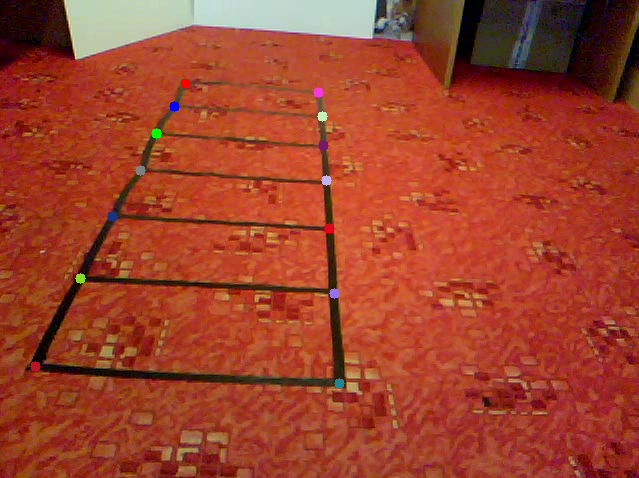
\includegraphics[width=\linewidth]{img/experiments/left-ladder.png}
\end{subfigure}
\begin{subfigure}{0.48\linewidth}
	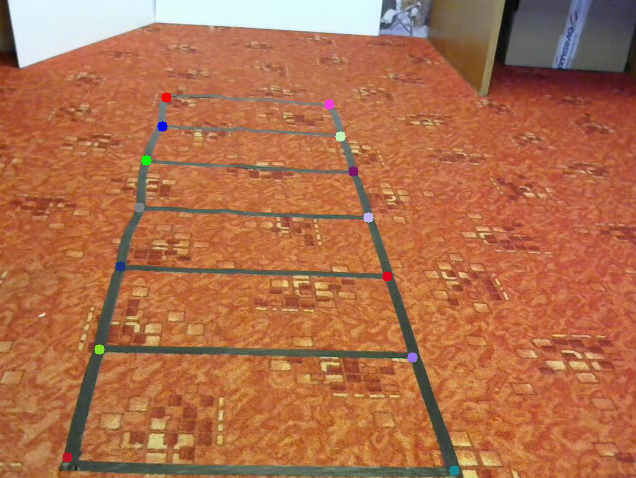
\includegraphics[width=\linewidth]{img/experiments/right-ladder.png}
\end{subfigure}
\caption{Selecting the points from the videos}
\label{fig:ladder_ground}
\end{figure}

\begin{figure}
\centering
\begin{tikzpicture}[]
	\draw (0, 0) -- (12, 0);
	\draw (0, 4) -- (12, 4);	
	\draw (0, 0) -- (0, 4);
	\draw (2, 0) -- (2, 4);
	\draw (4, 0) -- (4, 4);
	\draw (6, 0) -- (6, 4);
	\draw (8, 0) -- (8, 4);
	\draw (10, 0) -- (10, 4);
	\draw (12, 0) -- (12, 4);
	\node [right] at (0.1, -0.25) {200mm};
	\node [right] at (2.1, -0.25) {200mm};
	\node [right] at (4.1, -0.25) {200mm};
	\node [right] at (6.1, -0.25) {200mm};
	\node [right] at (8.1, -0.25) {200mm};
	\node [right] at (10.1, -0.25) {200mm};
	\node [right] at (12.1, 2) {400mm};
\end{tikzpicture}
\label{fig:grid}
\caption{Pattern used for experiments}
\end{figure}

\section{Full experiment}
\todo[inline]{nejaky full experiment s hybajucim sa objektom}

